\section{Results}
\label{sec:results}

The primary experiment is the Class~A search for a drifting, unresolved
spectral carrier: \NWinA{} fine-channel windows toward \NSysClassA{} systems.
Of those windows, \EdrNWinA{} are channelised finely enough on the criterion of
\S\ref{sec:statistic} to tell a drifting carrier from a stationary one. The
Class~B search for an unresolved spectral excess is secondary and carries no
drift discrimination: \NWinB{} coarse windows. Together they are the
\NWindows{} windows of the primary census. No event satisfied the confirmation
criterion set out in \S\ref{sec:summary}.

\subsection{Sensitivity: the power at which a carrier would have crossed
the threshold} \label{sec:pninetysel}

\emph{The median system, on its best window, would have produced a threshold
crossing from a carrier of $\EirpNinetySysMedA$\,W.} Each window's limit is
taken over the channels the attribution mask leaves, in the star's own rest
frame (\S\ref{sec:summary}): the finest windows were tuned to CO, a
\UmFineChanKHz\,kHz window spans \UmFineBwMHz\,MHz against a mask
\UmFineMaskMHz\,MHz wide, and \UmNWinAFull{} of the \NWinA{} Class~A windows,
the two finest among them, lie wholly inside it and constrain nothing. Across
the \NSysALim{} systems left with a constrained window the limits run from
$\EirpNinetySysLoA$ to $\EirpNinetySysHiA$\,W (Fig.~\ref{fig:classasens}),
\NSysEfifteen{} of them reach $10^{15}$\,W and the median Class~A
\emph{window} reaches $\EirpNinetyWinMedA$\,W; for \NSysALostName{} every fine
window is inside the mask and no limit is quoted. In \FcNBlock{} blocks whose
in-beam fields were recombined after the limits were computed, the search ran on
the recombined data, so the quoted limits there are conservative: for the
\FcNSys{} systems whose adopted limit such a block sets, by a median factor of
\FcMedFactor{} and at most \FcMaxFactor{}. Over the \EdrNWinA{} windows
in which the searched drift crosses a channel the search covers
\EdrUnionGHz\,GHz toward \EdrNSys{} systems, and restricting each
system to them gives a median \ScEdrMedPct{} per cent \ScEdrMedSense{}.

Carriers were injected at a random sub-channel phase and a random drift from
each window's own grid and recovered through the unchanged pipeline, through
the trigger and the localisation at the stellar position inside one execution
block. Nine in ten come back at $\EirpNinetyMultA\,P_{\rm trig}$ in Class~A,
$P_{\rm trig}$ being the bare $\LtCommonSnr\sigma$ of the window itself, and
that power is $\mathrm{EIRP}_{90}$; it does not depend on the brightness of the
control ring (Fig.~\ref{fig:strata}), and the correlator's spectral response is
carried by the injected tones and so sits inside it
(Appendix~\ref{app:conventions}). The \NCtrl-position spatial rank is not
charged against it: that would cost a further factor $\SensCostLike$, and in
\SensNRingHiUnres{} bright-ring windows it could not be met at any injected
power. Class~B carries its own factor, $\EirpNinetyMultB\,P_{\rm trig}$ from
\SensNToneCoarse{} carriers injected into \SensNInjCoarse{} coarse windows of
\SensNInjCoarseBlock{} execution blocks, which sets the limits for Barnard's
Star, Wolf~359 and Proxima. The calibration interval of the class factor,
$\times\SensFacLo$--$\times\SensFacHi$ (Table~\ref{tab:p90budget}), applies to
the median and the counts and not to any one window's limit: the median
system's limit carries it, $\TfMedCalLo$ to $\TfMedCalHi$\,W, so the second
figure of that median is set by the calibration and not by the depth of any
observation.

\emph{Every limit quoted here is nominal in one respect: it excludes
atmospheric decorrelation}, which a carrier injected into calibrated
visibilities does not suffer and a real one does. Measured block by block from
the phase rms the observatory records on each block's phase calibrator
\citep[\S\S10.4.11, 11.3.1]{ALMAHandbook} through the standard phase-scatter
relation \citep[Eq.~3]{Richards2022}, it leaves the median system's best window
optimistic by \NmDecSysMedPct{} per cent -- \SensDecorPct{} per cent for the
median window of the census, \SensDecorHiPct{} per cent above
\SensDecorHiGHz\,GHz, and \NmDecSysWorstPct{} per cent for
\NmDecSysWorstName{}. It is stated and not folded in because it is available
for \SensDecorNBlk{} blocks of \SensDecorNBlkTot{} only, the rest measurably
the harder ones, and folding it in where it is known would leave limits
neither corrected nor uncorrected. Table~\ref{tab:persys} gives it system by system
(Appendix~\ref{app:persys}). Applied there where a record allows it, it moves
the median limit above by \NmDecAdjShiftPct{} per cent -- inside the two
figures these powers are quoted to -- and takes the \NSysEfifteen{} systems
reaching $10^{15}$\,W to \NmDecAdjNEfifteen{}. No system's best window lies
above \SensDecorHiGHz\,GHz, so the high-frequency figure touches none of the
limits quoted here.

The primary-beam response at the star's own offset, the annual parallax the
phase centre omits and the smearing of a carrier within one integration are
divided out window by window, each bounded in Table~\ref{tab:p90budget} and
defined in Appendices~\ref{app:conventions} and~\ref{app:pbresp}. \emph{The
net bias on one limit is therefore of either sign}: the injected
profile's \InjShortPct{} per cent shortfall against the exact channel response
makes a limit conservative and the decorrelation makes it optimistic. In the
median window the first is larger and the quoted limit is conservative by
\NmNetConsPct{} per cent; at the ninetieth percentile of the systems' own best
windows the second is, and the limit is optimistic by \NmNetOptPct{} per cent
net of that shortfall -- \NmDecSysHiPct{} per cent before it -- rising to
\NmNetOptMaxPct{} per cent net and \NmDecSysWorstPct{} gross for
\NmDecSysWorstName{}.

\emph{Carriers were injected directly into \SensNInj{} of the \NWinA{} Class~A
windows, \SensNInjPct{} per cent, and the result transferred to the remaining
\SensNTransfer. That transfer is the dominant caveat on everything above.} The
injected windows are those of whole execution blocks drawn in a random order
and balanced by band and array, and over \RpNAxis{} properties they span the
central eight-tenths of the population, five of the six agreeing in the median
to \RpCovOtherPct{} per cent and the sixth, \RpCovWorstAxis,
$\times\RpCovWorstRatio$ noisier (Appendix~\ref{app:persys}). Only the ninety
per cent point in units of the window's own trigger power is carried across;
everything that turns it into a power is that window's own measurement. Across the injected windows that point ranges from
$\times\SensIndivFacLo$ to $\times\SensIndivFacHi$ of the adopted factor, with
\NmDispNTenth{} of the \SensNInj{} within a tenth of it. \emph{That
dispersion, and not the calibration interval above, is what one uninjected
window's own limit is uncertain by}. On the five properties that set the
reading -- band, channel width, array configuration, integration time and
block duration -- \NgNInterpWin{} of the \SensNTransfer{} transferred windows
lie inside the injected range on every one, and \NgNExtrapWin{} outside it on
at least one, where the range just quoted is not an empirical bound.
\NgExtrapTakeClause{}, and none is among the \NSysEfifteen{} systems reaching
$10^{15}$\,W. The best window was
itself injected into for \SmcNMeasSys{} of the \NSysALim{} systems, marked as
measured in Table~\ref{tab:persys}; for the other \SmcNEstSys{} the headline
limit is an estimate carrying that dispersion. \emph{The median quoted above
is therefore a calibration-transferred estimate and not a measured
sensitivity.}

\emph{A carrier that is not always radiating is penalised in proportion}: over
\DutyNTrial{} undrifted trials at duty cycles down to \DutyCycleMinPct{} per
cent the recovered amplitude followed the duty cycle to \DutyAttenDevPct{} per
cent, so a transmitter radiating a tenth of the time needs $\DutyPowFac\times$
the power quoted above, the joint drifting and intermittent case being
unmeasured.

\begin{table*}
\centering
\scriptsize
\caption{What sets $\mathrm{EIRP}_{90}$, and in which direction. The
calibration interval applies to the class-average factor and so to any
statistic over many windows; the spread between windows is an observed
dispersion and is the statement about one window; the signed terms are biases
and are not folded into an error bar (\S\ref{sec:pninetysel}).}
\label{tab:p90budget}
\setlength{\tabcolsep}{2pt}
% GENERATED by sens_r11.py -- do not hand-edit.
\begin{tabular}{@{}l@{~~}r@{~~}>{\raggedright\arraybackslash}p{0.61\linewidth}@{}}
\hline
 & value & what it does to the limit \\
\hline
Class-average completeness & $\times3.03$ & nine carriers in ten recovered at this multiple of a window's own trigger power. \emph{Measured} in the 49 Class~A windows injected directly and \emph{estimated}, at this factor, in the other 356 \\
\hline
\multicolumn{3}{@{}l}{\emph{Uncertainty on that calibration} (per cent), combined in quadrature} \\
The factor itself & $\pm2$ & sampling error of the pooled value over the 49 injected windows \\
Absolute flux scale & $\pm\BudFlux$ & the observatory's own band-dependent specification (\BudFluxSource): \BudFluxSpec, weighted over this sample's bands \\
Distance and visibility scale & $\pm\BudDistVis$ & the Gaia parallaxes, which enter as $d^{2}$, and the block-to-block visibility scale \\
\emph{Combined} & $-11/+11$ & $\times0.89$--$\times1.11$ on the factor, and so on the median limit and on the system counts; $\pm\BudCombWorst$ for the \BudNHiWin{} Class~A windows in \BudHiBandWord~\BudHiBands, at \BudHiGHzList\,GHz \\
\hline
\multicolumn{3}{@{}l}{\emph{Spread between windows}. An observed dispersion, not an error bar.} \\
Window to window & $\times0.80$--$\times1.58$ & the 49 injected windows resolve 2.41--4.80\,$P_{\rm trig}$ individually, \NmDispNTenth{} of them within a tenth of the pooled value and the second largest at $\times\NmDispSecond$. This, and not the interval above, is what an estimated limit is uncertain by; it is wider, and it applies to \SmcNEstSys{} of the \NSysALim{} systems \\
\hline
\multicolumn{3}{@{}l}{\emph{Applied} window by window where a record allows it and bounded where none does, and so not combined with the above.} \\
Intra-integration smearing & $\times1.00$--$\times\SmcFacWorst$ & a carrier sweeps through part of a channel within one integration and the injected ones do not: $\eta_{\rm smear}$ at the drift that sets a ninety per cent point, from each window's own integration length where it is recorded (\SmcNMeas{} windows) and from the longest delivered anywhere where it is not (\SmcNBound) \\
Primary beam & $\times1.00$--$\times\NmBeamFacWorst$ & the star is not at the pointing centre, so each limit is divided by the response at its own offset, on the full width the observatory documents. Nothing in the median window; the \BmNAboveTenPct{} windows furthest off-axis carry the departure of that form from a blocked circular aperture, up to \BmModelMaxPct{} per cent, as a one-sided systematic \\
Annual parallax & $\times1.00$--$\times2.06$ & the phase centre omits it, so each limit is divided by the amplitude a compact source retains at its own displacement, a median \PxaLossMedPct\,per cent on the \PxaNWin{} windows carrying a parallax record; on the other \PxaNMissing{} the loss is bounded (Appendix~\ref{app:pbresp}) \\
\hline
\multicolumn{3}{@{}l}{\emph{Signed terms}. A bias is not an error bar and is not added to one.} \\
Channel response & $\times\RpRespFac$ & one over the share of a channel-confined carrier the peak channel keeps. Carried by the injections, so already inside the completeness above, which is this factor times a margin of $\times\RpMarginNinety$ over the nominal trigger \\
\quad its residual & $+\InjShortPct$ & the injected profile falls short of the exact response: \emph{conservative} \\
Decorrelation & $+0/+\NmDecSysWorstPct$ & measured block by block from the phase rms the observatory records on each block's phase calibrator, which an injected carrier does not suffer and a real one does. One-sided, and a floor. A median $+\NmDecSysMedPct$ on the systems' best windows, $+\SensDecorHiPct$ above \SensDecorHiGHz\,GHz, and more than $+\SensDecorTailLevelPct$ in \SensDecorTailPct{} per cent of windows \\
\hline
\end{tabular}

\end{table*}

\begin{figure}
\centering
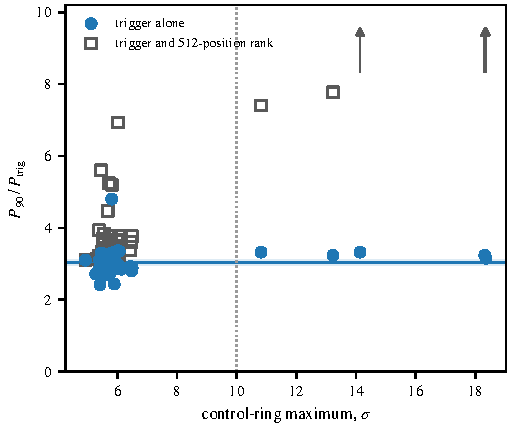
\includegraphics[width=\columnwidth]{figures/sens_ring.pdf}
%% ★ v4.26 (r25-captions): 9 printed lines -> R1 §7's limit of about six.
%% \S\ref{sec:pninetysel} above already carries every statement removed:
%% that the value does not depend on the ring's brightness, what charging
%% the rank would cost, and the bright-ring windows that cannot meet it at
%% any injected power -- the arrows.  \SensRingRule had this caption as its
%% only citation site, so the dotted line's threshold MOVED into that
%% paragraph rather than being dropped.
\caption{Why one completeness factor serves the whole class. The
\SensNInj{} directly injected Class~A windows at the power recovering nine
carriers in ten, each against its own \NCtrl-position ring maximum: no trend
with the ring. Filled, the criterion adopted here, pooled value as line and
band; open, the rank charged too, arrows where no power meets it; dotted, a
resolved ring.}
\label{fig:strata}
\end{figure}

\begin{figure}
\centering
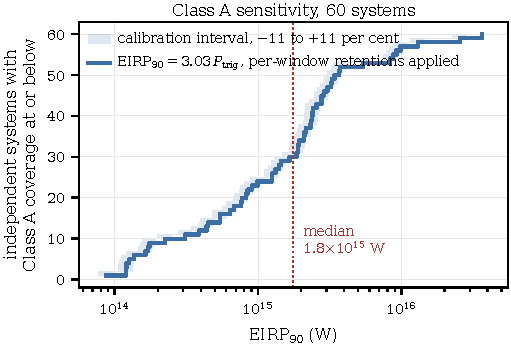
\includegraphics[width=\columnwidth]{figures/classa_sensitivity.pdf}
%% ★ r27 (R2-D10): panel (b), the Class A systems with a separated repeat
%% counted by system, duplicated Fig.~\ref{fig:confcov}b and LEAVES; Fig. 5
%% itself is protected and stays, one panel, one column.  Its four assertions
%% (\ZcConfSysDay, \ZcConfSysYr, \ZcNoRepSys, NSysClassA) still run in
%% make_fig_classa_sens.py.
\caption{\textbf{Single-epoch trigger completeness of the carrier search}:
the cumulative number of systems whose best window reaches a given
$\mathrm{EIRP}_{90}$, each window's own retentions applied and atmospheric
decorrelation excluded, the calibration interval of
Table~\ref{tab:p90budget} shaded. Confirmation needs a separated repeat,
which no power buys and which \ZcNoRepSys{} of the \NSysClassA{} systems lack
(Fig.~\ref{fig:waterfall}b; \S\ref{sec:mmdifferent}).}
\label{fig:classasens}
\end{figure}

\subsection{The nearest stars: Barnard's Star and Wolf~359}
\label{sec:barnardswolf}

Barnard's Star is the second-nearest stellar system and Wolf~359 the third if
brown dwarfs are excluded. To our knowledge these are the first millimetre
or submillimetre technosignature limits for either. Radio searches of the
nearest stars have worked at centimetre wavelengths
\citep{Enriquez2017,Price2020,Margot2023}. Both are non-detections, and
\emph{both limits come from the secondary Class~B experiment and not from the
carrier search}: the archive holds only coarse Band~6 windows toward these
stars. On the $\mathrm{EIRP}_{90}$ convention of \S\ref{sec:pninetysel}
Barnard's Star reaches $\EirpNinetyBarnLo$--$\EirpNinetyBarnHi$\,W over
\NWinBarn{} windows and Wolf~359 $\EirpNinetyWolfLo$--$\EirpNinetyWolfHi$\,W
over \NWinWolf.

\subsection{Threshold crossings and how each was disposed of}
\label{sec:technosearch}

Of the windows the search covers -- the \NWindows{} of the primary census and
the archival-tail blocks beside them -- \EvNCrossRaw{} hold a cell reaching
$T\geq5$ at the stellar position. \EvNCrossFlag{} lie in the one execution
block that fails the quality criterion of \S\ref{sec:bdblock}, so the
population that characterises the search is the \EvNCrossQp{} in
quality-passing data and those \EvNCrossFlag{} are reported beside it. The
molecular-line mask is $\pm\MaskHalfKms$\,km\,s$^{-1}$ wide in each star's own
rest frame and places \MkNCoinc{} of the \EvNCrossQp{} within that distance of
a catalogued transition. A further \SoNCrossWord{} fall on transitions of a
species no debris disc has been shown to carry. The mask does not hold those
transitions, so they stay unattributed, with their offsets reported
(Appendix~\ref{app:linemask}). That leaves \EvNAttrQp{} crossings attributed
and \EvNUnattrQp{} unattributed. The attributions are kinematic and not an
accident of bandwidth. In the frame the correlator delivered, the crossings
with a measured peak frequency crowd onto the transitions these setups were
tuned to, far more tightly than a free landing on their own grids would put them
(Appendix~\ref{app:rfi}). Of the unattributed, \EvNRankQp{} outrank all
\NCtrl{} control positions of their own window, and neither of those two is
present again at the cell its own discovery predicts. No crossing survives the chain, and this
survey reports no detection; the crossing ledger, which accompanies this paper
as data, lists every one.

\emph{Anything bright in a window hides a weaker carrier behind it, so the
weaker cells were sought too.} The de-drifted statistic is retained in every
channel. Behind a window's tabulated crossing, its largest cell, weaker
above-trigger cells can therefore be read as well, neighbouring channels
counting as one. There are \CkNSecondaryWord{} of them, of which \CkNSecUnattrWord{} are
unattributed and \CkNRecurWord{} reaches the trigger in any of the covering
blocks the recurrence test reads. Cells are counted in the controls too.
Outside the mask the star holds slightly more of them than a control position
at every level below the trigger, with no step where a carrier search would put
one (Appendix~\ref{app:falsealarm}, \S\ref{sec:trigunif}).

\subsubsection{The unattributed count is what the control positions predict}
\label{sec:trigunif}

The trigger is a threshold on a statistic and not a false-alarm rate -- the
searched channel\,$\times$\,drift cells per window span \TuCellsDecades{}
decades -- so the chance count is measured window by window over the \CeNWin{}
Class~A windows of the census, with one condition on both sides of the
comparison: a cell at the stellar position that reaches the trigger and that
the line mask does not attribute (Appendix~\ref{app:falsealarm} gives the
method). These fields' own control positions predict \CeExp{} unattributed
Class~A crossings and \CeObs{} are found. A count that large or larger arises
by chance with probability \CeProbNull{} -- a probability conditional on the
control positions being a model of the stellar position, the one assumption
the searched data cannot test. Calibrated instead at the stellar-to-control
ratio \CeNear{} measured just below the trigger, as a sensitivity test, the
expectation is \CeExpNear{} at $P=\CeProbNear$, and the whole-beam conclusion
of no significant excess is unchanged under it. A calibration error varying
with frequency would raise the star and not its continuum-free controls, but
the least demanding window would need \CyEpsMinPct{} per cent of its star's
continuum to reach the trigger, and the mild excess below it runs the wrong way
with continuum brightness, \CkRatioContBright{} against \CkRatioContFaint{} over
the \CkNContWin{} windows with a photospheric estimate.

Both sides are read over the whole primary beam \S\ref{sec:statistic} defines,
the statistic Equation~\ref{eq:tstar} specifies; a narrower field drops the
integrations whose pointing falls outside it and with them on-source time and
real signal. Read over such a field on both sides the same comparison gives
\FrNarrowObs{} against \FrNarrowExp{} at $P=\FrNarrowProb$, reported beside the
first and not in place of it. Both geometries are applied uniformly to every
window and to both sides, but neither was nominated as the primary before the
counts were compared, and the choice between them was made after the counts had
been seen. The whole beam shows no significant excess and the narrower field a
nominal one; corrected for the \FrNRead{} readings tested the smaller
probability is \FrTwoTrialP, so neither departs from chance at the
\CeAlphaPct{} per cent level -- a correction that assumes only these \FrNRead{}
choices were made, and so does not settle the disagreement. The interpretation
therefore depends to some extent on the extraction geometry, and neither
reading establishes a population of non-astrophysical transmitters.

The observed count is compatible with a background estimated empirically from
these same fields, which is not a null distribution established independently
of the model. What the comparison could not have rejected is \CeAddLim{}
further crossings against those control positions, \FrNarrowAddLim{} on the
narrower reading -- conditional on that model, a count of crossings and not of
transmitting systems, since several crossings could come from one source, and
not an occurrence rate (Appendix~\ref{app:falsealarm}). Each crossing is
tested individually by the recurrence test of \S\ref{sec:etacrv}.

\subsubsection{One execution block accounts for four of the crossings}
\label{sec:bdblock}

\BdNCross{} crossings belong to \BdStar{} (\BdAlias), all of them in one ACA
execution block, \texttt{\BdBlock}, whose whole field is above threshold.
Of its \BdNCtrl{} control positions, \BdNCtrlAbove{} exceed $T=5$, where the
median of a window's own control ensemble is \BdSurvCtrlMed{} across the
survey. Its
single-integration noise is as predicted, but it does not integrate down: a
jackknife on the channel mean stands \BdJackRatio{} times above thermal while
neighbouring channels stay uncorrelated. That describes a residual persisting
from one integration to the next and differing from channel to channel
(Appendix~\ref{sec:blockquality}). Equation~\ref{eq:tstar} divides by the noise
of the stacked spectrum, which falls as the root of the integration count. A
residual that does not average down therefore accumulates along a drift track faster than
the denominator grows, and it does so at every position in the field.
\emph{The field is inflated and the star is not}: the \BdNSibling{} sibling
executions of the same field, array and setup produce no crossing, and in
all four a control stands above the star, \EvFlagNgeLo--\EvFlagNgeHi{} of the
\BdNCtrl{}. The criterion fails this block and no other at any threshold between
it and the next most extreme block, so its \BdNCross{} crossings are reported
apart from the \EvNCrossQp{} and Appendix~\ref{app:rfi} carries what the block
might instead be. Milder cases are not unique to it: read window by window the
same diagnostic flags \DqNWin{} windows in \BkFlagNBlock{} blocks, and the
\BkFlagNCrossOther{} flagged crossing outside this block -- \BkFlagOtherStar{}
-- is withheld from the amplitude-dependent tests for it too.

\subsubsection{Stellar flares are excluded by a broadband prediction}

Known flare stars are in the sample, but a millimetre flare raises every
channel of a window alike. One able to produce a single-channel crossing at
the trigger must therefore produce a $5\sqrt{N}\sigma$ continuum event in the
same integrations. With $N$ the window's own channel count,
\FlNChanLo--\FlNChanHi{} across the windows holding a crossing, that prediction
runs \FlPredLo--\FlPredHi$\sigma$. The observed continuum statistic has a
median of \FlObsMed{} over the \FlNCont{} crossings with a recoverable
measurement, and $|Z|<3$ in \FlNQuiet{} of them. A flare origin in fact needs more than
that, because the per-integration median along frequency
(\S\ref{sec:statistic}) removes a flat continuum before the search. Only a
flare's departure from flatness across the band can reach a single channel. The
prediction is therefore a floor on what such an origin requires and the contribution
measured below is a bound on what one supplies. One block settles it:
\FlEgStar{} \texttt{\FlEgEb} holds both a crossing ($T_\star=\FlEgT$) and the
millimetre flare of \citet{MacGregor2020}. That flare contributes
\FlEgContrib$\sigma$ to the single-channel statistic. It raises the continuum
at $Z=\FlEgContZ$, while the crossing's own de-drifted track reaches
$Z_{\max}=\FlEgTrackZ$.

\subsection{$\beta$~Pictoris: an astrophysical positive control, and the
obstacle it identifies} \label{sec:bpicval}

\emph{A search that finds nothing must show that it could have found something,
and the survey's strongest features show exactly that.} The pipeline recovers
the $\beta$~Pictoris circumstellar carbon monoxide without being told the disc
is there. It does so in two rotational transitions and in \CsBpCoBlocks{}
execution blocks spanning \BpBaselineYr\,yr, drawn from \CsBpCoSess{} observing
sessions, the closest two \CsBpCoSepMinD\,d apart. In \NStageOneBpicEb{} of the
blocks the star also outranks every control, but the identification is
kinematic and does not rest on those statistics. Carried through the frame
chain to the barycentre at each block's own epoch and then to the star's rest
frame, all \BpicPanelNCo{} crossings lie within \BpicDvCoHi\,km\,s$^{-1}$ of the
stellar systemic velocity. They lie in the two lowest CO transitions of a star
with mapped circumstellar CO \citep{Dent2014,Matra2017}. The Band~3 peaks agree
across blocks to \BpRecThreeTuneChanMax{} channel once each block's own tuning
is removed. The alternative reading requires a transmitter placed by coincidence
at matched offsets from two CO transitions of one star. It is also the control
that shows the recurrence test of \S\ref{sec:etacrv} working in the positive
direction. Every flagged feature is recovered in another execution block and
each transition in a block of another session as well, the screened Band~6
window returning $T_\star=\BpRecTTwo{}$. A non-recurrence elsewhere means
nothing unless the same machinery recovers a repeat where one exists.
\emph{One of those blocks is a counterexample, and it is the more useful half of
the control}. In block \texttt{\BpCtrlBlock}, Band~\BpCtrlBand, the control ring
reaches \BpCtrlRingMax{} against \BpCtrlStar{} at the star. Several of the
\NCtrl{} control positions therefore exceed the stellar statistic, and the
spatial rank disfavours a window holding carbon monoxide known to be real and
centred on the star. The disc is resolved on the scale of the primary beam in that
configuration. That is the geometry the statistic is built to reject, so the
rank tests compactness and not authenticity, and on a real extended source it
errs conservatively (Fig.~\ref{fig:bpiccontrol}). Extended emission is in fact identified by the
\emph{level} of the control ring and not by the star's rank against it. That
is why the window-level flag of Appendix~\ref{sec:blockquality} is defined on
the ring's median. Appendix~\ref{app:linemask} gives the complementary case,
HD~48370, whose crossing matches the prominent CO($2{\to}1$) that
\citet{Cataldi2023} report toward the source and flag as possible cloud
contamination. Its control ring rises with the star, as emission filling the
primary beam does. The mask that removes
this emission covers \FrNSpec{} species and costs \MkMaskAPct{} per cent of the
Class~A union bandwidth, and it is nevertheless the single most productive test
in the chain (Appendix~\ref{app:linemask}). \S\ref{sec:mmdifferent} draws the
lesson.

\subsection{The two crossings that lead their own control fields}
\label{sec:vistest}

Two crossings reach a stellar statistic above every one of the \NCtrl{}
control positions in their own window, and neither is a detection: \EvAStar{}
at \RqFreqSx\,GHz and \EvBStar{} at \RqFreqCp\,GHz, both in Band~\EvABand{} and
in the star's own rest frame (the delivered frequencies are in the ledger),
tabulated in Table~\ref{tab:cand} and the first drawn in Fig.~\ref{fig:event}.
Their control rank says which crossing was examined first and disposes of
nothing (\S\ref{sec:method}): were the stellar and control positions
exchangeable, the star would lead all \NCtrl{} with probability $1/\RkCtrlDen$,
so \RkExpLead{} of the \RkNUnattr{} unattributed crossings would do so by chance
and two or more with probability \RkProbTwo, against
\RkHoLead{} of \RkHoN{} in the reserved blocks and \RkOosLead{} of \RkOosN{}
beyond 40\,pc, and the positions are not exchangeable (\S\ref{sec:summary}).
\EvBStar's crossing lies $\EvBDv$\,km\,s$^{-1}$ from \EvBLine, a note and not a
disposition (Appendix~\ref{app:linemask}). A visibility-domain fit, made for
\LgNFit{} of the \NCross{} crossings and consistent with a point source at the
star for \LgNLocalCor, excludes neither, injected sources in the bin these two
occupy returning ${\rm Re}/\sigma=\RsevReAtFiveMeanA\pm\RsevReAtFiveSdA$; of
the \NCtrl{} control positions, \RcNRetCtrl{} retain a dynamic spectrum and
\RcNVisCtrl{} are reachable in the visibilities. Neither crossing is present
when the same stellar-frame frequency is observed again: the nearest covering
block, \RcSxNearH{} and \EvBDeepH\,hours from each discovery, bounds a
returning carrier below \RqNearFracSx{} and \RqNearFracCp{} of the discovery
amplitude, and every covering block combined deepens that to \RcSxFive{} and
\RcCpFive{} over \RqSpanDSx{} and \RqSpanDCp\,days. Either reading covers half
a channel in the star's frame, $\pm\RqDispSx$ and $\pm\RqDispCp$\,km\,s$^{-1}$,
which each carrier's own fitted drift would cross in \ZtSxLeaveSec{} and
\ZtCpLeaveSec{} seconds, so the test asks for a return to that frequency and not
a stability at it (\S\ref{sec:etacrv}); $T_{\rm rep}$ is one cell at one trial
and may be negative, and the recovery chance in brackets, at the discovery
amplitude, is biased high. At the faintest amplitude consistent with each
crossing having been found the criterion would have recovered a persisting
carrier with calculated probability \RqPowerTrigSx{} and \RqPowerTrigCp, and
injected carriers measure \HjMeasSx{} and \HjMeasCp, so for \EvBStar{} the
silence is not an exclusion. The readings behind each bound -- the largest single epoch,
the maximum over every drift and the value over the matched registration
tolerance -- are in \texttt{candidates/repeat\_epoch\_readings.csv} of the data
archive \citep{SIdeposit}.


\subsection{Recurrence, applied across the unattributed crossings}
\label{sec:etacrv}

Because a transmitter in orbit changes its line-of-sight velocity between
epochs, the broad test is whether anything above the trigger is present again
anywhere in a covering window, at every drift of the grid. That window is $\pm\WdHalfKms$\,km\,s$^{-1}$ wide in the median case, wider
than the $\pm\EcVexcKms$\,km\,s$^{-1}$ an orbit at the grid's
\WdAGrid\,m\,s$^{-2}$ ceiling can produce about any star here. \WuNWinExc{} of the \WuNWin{} distinct covering windows hold a
statistic above the trigger, against the \WuExpWin{} chance predicts
($P=\WuProbWin$, or \WuExpWinCtrl{} at $P=\WuProbWinCtrl$ when the rate
comes from each window's own control positions instead of its cell count;
Appendix~\ref{app:falsealarm}) -- a marginal excess, and every one of those
windows holds a crossing the ledger already lists, so this comparison re-reads
the trigger-level excess of \S\ref{sec:trigunif} rather than adding a
recurrence to it. \WuNWinExcTwo{} of the \WuNWinExc{} are toward
\WuTwoStars{} (\S\ref{sec:twostars}); over the remaining \WuNWinRest{} windows
the reading is \WuNWinRestExc{} against \WuExpRest{} at $P=\WuProbRest$
(Appendix~\ref{sec:pairacct}). No recurrence is established here, and none is excluded.

Table~\ref{tab:pairs} asks of the \TjNPair{} pairs of crossings inside that
interval, across \TjNStarPair{} stars, whether one transmitter could have
produced both (Appendix~\ref{sec:pairacct}). Constant line-of-sight acceleration means
$\dot\nu_1=\dot\nu_2$, and the two fitted rates differ by more than the grid's
own rate resolution in \TjNUneqDrift{} of the \TjNPair{} pairs. In
\TjNPower{} of them the epochs are close enough together that the offset such
a trajectory predicts is tighter than the window searched about the cell, and
those \TjNPower{} fail a drift changing at a constant rate as well. The weaker and
safer question, whether any trajectory inside the searched grid joins the two,
separates \TjNExcl{} pair, \EcGridStar's two crossings needing \EcGridFactor{}
times the grid's ceiling between them; the other \TjNOpen, \TjNOpenPlain{}
\emph{open} and \TjNPairEdge{} \emph{edge-limited}, are neither a confirmation
nor an exclusion, since the comparison can reject a drifting carrier and cannot
accept one.

\emph{A third reading is a check on line attribution, and not a test of
persistence}: the single cell each discovery predicts at the repeat epoch,
maximised over nothing, which is right for an emitter at rest in the star's
frame, as a line is, and wrong for a carrier: the fitted line-of-sight
accelerations of the \RcNExcl{} run from \ZtALosLo{} to \ZtALosHi\,m\,s$^{-2}$
in the observatory's frame and from \EgExStarALosLo{} to \EgStarALosHi{} in the
star's own -- the two frames differ by the observatory's own acceleration and
so by at most \EgFrameALosMax\,m\,s$^{-2}$ -- and a drift that size carries a
carrier out of the half-channel the reading covers in \ZtLeaveSecLo{} to
\ZtLeaveSecHi{} seconds, a median of \ZtLeaveSecMed. The shortest interval
any of them has between its two epochs is \ZtGapOverLeaveMin{} times the
longest of those residences. It is therefore reported here as a \emph{line-recurrence check}, and
no crossing is called excluded on it. Nor could it be extended to a carrier
by carrying that carrier's own fitted drift forward: the half grid step the
drift is resolved to holds the predicted cell inside half a channel for a
median \ZtRegHoursMed\,h (\ZtRegHoursLo--\ZtRegHoursHi), which \ZtNRegNear{}
of the \RcNExcl{} exceed before their nearest repeat, and it displaces the
cell by a median \ZtRegChanMed{} channels there and \ZtRegChanFarMed{} over
the longest baseline. It works in that direction: \MkAttrRecur{} of the
\MkAttrTested{} crossings attributed to carbon monoxide recur in another
session, the strongest recovery of each \QcSepMinD--\QcSepMaxD\,d away --
\RqNRecurDisc{} in the disc of \RqRecurDiscStars{} and \RqNRecurCloud{} in
interstellar gas toward \RqRecurCloudStars{} (Appendix~\ref{app:linemask}) --
but every disc recovery has $T_\star\ge\RqRecurDiscTLo$, and the
\MkAttrExcl{} not recovered are the two faintest, both at
$T_\star=\RqNearTrigT$. On the \RcNExclPoss{}
unattributed crossings whose predicted cell could be read it returns nothing:
none is present at its predicted cell, the largest single-block reading at the
carried drift being \RcTMatched{}, and \RcTMax{} the largest at any drift of
the grid, against a trigger of \StageNullTrig; the remaining
\RcNNoSpec{} of the \RcNTested{}, toward \RcUntStar{} at \RcUntFreq\,GHz,
retains no discovery spectrum, so there is no amplitude to carry to a repeat
epoch and no reading of its own. Over the \RcNExcl{} crossings whose repeat
coverage carries an amplitude bound, a carrier returning to within half a
channel is bounded to a median \RcFracMed{} of the discovery amplitude and
\RcFracMax{} at the weak end, where \HjNPowerLo{} are too shallow to test at the
trigger amplitude; no disposition depends on the cell's registration, on the
anchor along the discovery track or on the threshold (Appendices~\ref{sec:nullscatter} and~\ref{sec:regbudget}). No crossing satisfies the confirmation criterion of
Table~\ref{tab:quantities}; the repeat coverage holds the marginal excess of
above-trigger windows given above, concentrated in \WuTwoStars; and no reading here
bears on a transmitter whose apparent frequency or acceleration changes
between epochs by more than these readings accommodate.


\subsubsection{The reserved hold-out and the control beyond 40\,pc}
\label{sec:holdoutsearch}

Three sets of execution blocks enter no census statistic
(Table~\ref{tab:blockledger}); each was searched with the same pipeline, every
compact-array block on the annulus of its own dish (\S\ref{sec:statistic}), and
each is reported here as a search. The \emph{hold-out} is \HoNBlock{} blocks,
\HoNWin{} windows, \HoNStar{} stars and \HoHours\,h on source, set aside by the
identifier rule of Appendix~\ref{sec:heldout} and sharing no execution block
with the census. It contains \HoNCross{} threshold crossings, the strongest at
$T_\star=\HoTMax$, none of them outranking its own control positions. Of
the \HoNTested{} tested for recurrence on the same code path exactly one is
present again -- a molecular line, so the test works in the positive direction
here as well, at $T_{\rm rep}=\HoRecTRep$ -- while for every other tested
crossing the repeat coverage bounds a carrier returning to the predicted cell
to \HoFracMax{} of the discovery amplitude or less. The \emph{archival extension}'s \LdgExtWin{}
windows in \LdgExtEB{} blocks hold \QxObsCross{} threshold crossings, every one
in a fine-channel window. Of these, \QxObsAttr{} lie inside the mask in their
own star's frame and \QxObsUnattr{} outside it, against \QxLam{} predicted by
chance (Appendix~\ref{app:falsealarm}). The chance of \QxObsUnattr{} or more is
\QxPGe{}. A sample this size could have shown a shortfall and does not,
$P(0\,|\,\QxLam)=\QxPZero$. The \emph{control beyond 40\,pc} is \OosNBlock{}
blocks and \OosNWin{} windows toward \OosNStar{} stars,
\OosHours\,h on source, holding \OosNCross{} crossings, the strongest at
$T_\star=\OosTMax$ and none outranking its own controls; the set is read in the
sky frame, supports no limit and shows only that the pipeline behaves the same way on
fields beyond the sample. The hold-out crossings are released row by row with
the catalogue, on the columns of the crossing ledger.

%% Numbers are generated, not
%% typed: every \Tw... macro is written by twostars_r27.py (round 992), which
%% also writes tab_twostars_r27.tex.
\subsection{HD~14055 and \BkAlmaName}
\label{sec:twostars}

Of the \WuNWinExc{} covering windows above the trigger, \TwNWinExcTwoWord{}
are toward these two objects; Table~\ref{tab:twostars} is every crossing
either of them holds.

They are also the two most heavily observed objects in the survey, holding
\TwWinASharePct{} per cent of the Class~A census and \TwNWinTwo{} of the
\WuNWin{} covering windows, so \TwExpTwo{} of the \WuExpWin{} expected
exceedances are theirs before anything is looked at. Taken one at a time the
two part company. HD~14055 holds \TwNExcHD{} against \TwExpHD{} expected
($P=\TwProbHD$; the control positions of its own windows predict
\TwExpCtrlHD): its concentration is its exposure. \BkAlmaName{} holds
\TwNExcJx{} against \TwExpJx{} and \TwExpCtrlJx{} on the two nulls
($P=\TwProbJxRaw$), a real local excess -- though it is the most
discrepant of the \TwLookNStar{} objects compared and was picked out for
being so: chance puts some object that far out in \TwLookPct{} per cent of
realisations.

Nothing about HD~14055's fields is unusual: the median of a window's control
ring over the median of its own class is \TwRingQHD{} for its windows,
against \TwRingQSurv{} for the survey and \TwBlockQMax{} for the one block
the quality criterion rejects (Appendix~\ref{sec:blockquality}). Its setups
are continuum ones, the nearest masked transition to any window centre
\TwHDCenMinKms\,km\,s$^{-1}$ away, and its crossings lie
\TwHDMaskLo--\TwHDMaskHi\,km\,s$^{-1}$ from CO or $^{13}$CO in its own frame. Its \TwHDNBlockCensusWord{} catalogued crossings come from blocks of a single
programme taken within \TwPairCensusSpanD\,d of each other, and
Table~\ref{tab:pairs}'s \TwPairSpanD\,d baselines come from its two
archival-tail crossings; the \TwHDNDeep{} epochs that carry the inverse
variance there are follow-up blocks outside the primary census, and on
them a carrier persisting at the discovery amplitude is excluded at
\TwHDExclA{} and \TwHDExclB$\sigma$. \TwHDNEdgeWordCap{} of its drifts lie on their grid's
outermost trial and are lower bounds, $|a_{\rm los}|\ge\TwHDEdgeALos$ and
$\ge\TwHDEdgeALosHi$\,m\,s$^{-2}$ -- at the top of the range searched, where
\S\ref{sec:statistic}'s caveat applies, and the reason \TwNPairEdgeHDWord{} of this
star's pairs in Table~\ref{tab:pairs} are edge-limited.

\BkAlmaName{} is a serendipitous dwarf \TwPbJx{} arcsec off the phase centre
of fields pointed at the Lupus clouds, in \TwOnSrcJx\,s snapshots. Its
CO($2\to1$) crossing is the only one of the \TwNCrossBoth{} sitting on a line
the observers tuned to: window centred \TwTunedCenKms\,km\,s$^{-1}$ from CO,
fitted drift \TwStepMin{} of a grid step from zero where every other is
\TwStepNext--\TwStepMax, and a control ring reaching $T_\star=\TwCtrlMaxJx$
against \TwTStarCtrlJx{} at the star -- cloud emission filling the field. The
star has no measured systemic velocity and the frame chain takes zero
(\S\ref{sec:statistic}), so the attribution of all \TwSweepNJxWord{} was recomputed over
$\pm\TwSweepHalfKms$\,km\,s$^{-1}$, wider than any systemic velocity adopted
here. \TwSweepNChangeJxWordCap{} changes: the CO crossing leaves the mask above
$v_{\rm sys}=\TwSweepVCrit$\,km\,s$^{-1}$, where its reading in the local
standard of rest, \LsLupDv\,km\,s$^{-1}$ from a catalogued cloud line, holds
anyway (Appendix~\ref{app:linemask}). The other \TwSweepNUnchJxWord{} never enter the
mask at any velocity of the sweep, the closest approach of any of them to a masked
transition being \TwSweepClosestKms\,km\,s$^{-1}$.

What is left is \TwNExcJxWord{} windows where \TwExpJx{} were expected, on \TwJxNCrossExcWord{}
crossings between \TwJxExcBandLo{} and \TwJxExcBandHi\,GHz in
\TwJxNBlockExcWord{} of this object's \TwJxNBlockWord{} blocks: ordinary control
rings, drifts far from zero, and a visibility fit placing
\TwJxNLocalExcWord{} of the \TwJxNCrossExcWord{} at the star and
\TwJxNNotLocalExcWord{} not. A transition of the \TwWideNSpecies-species list lies
within \TwWideDvMax\,km\,s$^{-1}$ of every row of Table~\ref{tab:twostars},
which \TwWideNTrans{} transitions guarantee and which identifies nothing. We
have no explanation, and these are the two objects a repeat observation
should point at -- HD~14055 for drifts that are lower bounds,
\BkAlmaName{} for a radial velocity and one deeper epoch at
\TwJxExcBandLo--\TwJxExcBandHi\,GHz.

\begin{table}
\centering
\caption{\textbf{Every crossing toward HD~14055 and \BkAlmaName.} Rates are
in the observatory frame; $\ge$ and $\le$ mark a fit on the grid's outermost
trial.}
\label{tab:twostars}
\scriptsize
%% GENERATED by twostars_r27.py -- do not hand-edit.
\begin{tabular}{@{}r@{~}r@{~}r@{~}l@{~}r@{~}r@{~}r@{}}
\hline
$\nu_\star$ & $T_\star$ & $\dot\nu_{\rm obs}$ & nearest masked & $\Delta v_\star$ & $\Delta v_{225}$ & ${\rm Re}/\sigma$ \\
(GHz) & & (Hz\,s$^{-1}$) & transition & (km\,s$^{-1}$) & (km\,s$^{-1}$) & \\
\hline
\multicolumn{7}{@{}l}{\emph{HD~14055}} \\
331.155 & 5.08 & $\le\!-3976$ & $^{13}$CO($3$--$2$) & $+514$ & $-1$ & $+4.4$ \\
331.703 & 5.28 & $+1104$ & $^{13}$CO($3$--$2$) & $+1012$ & $-5$ & $+5.1$ \\
331.766 & 5.58 & $-3857$ & $^{13}$CO($3$--$2$) & $+1069$ & $-12$ & $+5.0$ \\
344.452 & 5.01 & $-2589$ & CO($3$--$2$) & $-1166$ & $+4$ & -- \\
344.696 & 5.17 & $-2426$ & CO($3$--$2$) & $-953$ & $-3$ & $+4.8$ \\
345.007 & 5.18 & $+1769$ & CO($3$--$2$) & $-684$ & $+2$ & $+4.6$ \\
345.430 & 5.45 & $+2584$ & CO($3$--$2$) & $-317$ & $-3$ & -- \\
345.522 & 5.19 & $\ge\!+4184$ & CO($3$--$2$) & $-238$ & $+1$ & $+5.0$ \\
\hline
\multicolumn{7}{@{}l}{\emph{\BkAlmaName}} \\
216.204 & 5.23 & $-2198$ & SiO($5$--$4$) & $-1245$ & $-5$ & $-0.6$ \\
217.727 & 5.09 & $-983$ & H$_2$CO($3_{0,3}$--$2_{0,2}$) & $-680$ & $+3$ & $+1.8$ \\
218.669 & 5.05 & $-2023$ & H$_2$CO($3_{2,1}$--$2_{2,0}$) & $-125$ & $-6$ & $+4.5$ \\
218.892 & 5.09 & $+2373$ & H$_2$CO($3_{2,1}$--$2_{2,0}$) & $+181$ & $-15$ & $+4.7$ \\
230.539 & 5.41 & $-19$ & CO($2$--$1$) & $+2$ & $+2$ & $+4.4$ \\
347.189 & 5.01 & $-2581$ & SiO($8$--$7$) & $-122$ & $-7$ & $+4.6$ \\
\hline
\end{tabular}

\end{table}

\begin{figure*}
\centering
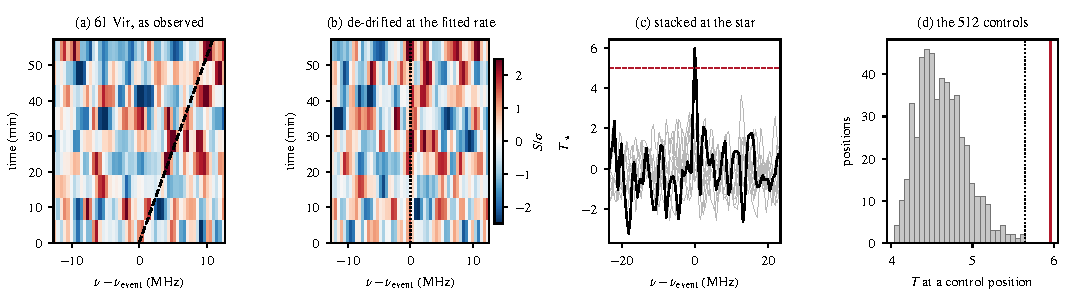
\includegraphics[width=\textwidth]{figures/event_crossings.pdf}
\caption{\textbf{The strongest unattributed crossing of the quality-passing
data, and the control field it leads.} Frequencies are in the star's rest
frame.
\emph{(a)}~The dynamic spectrum at \EvAStar's position around the crossing
at \RqFreqSx\,GHz, observed \EvADate, the fitted drift of
\EvADrift\,Hz\,s$^{-1}$ dashed, \EvANInt{} integrations binned into
\EvANBin{} and plotted in units of each bin's noise.
\emph{(b)}~The same rows shifted by that drift.
\emph{(c)}~The de-drifted stack at the star (black) and at the
\RcNRetCtrl{} control positions with retained dynamic spectra (grey), in
units of its own noise, the trigger dashed. \emph{(d)}~The same statistic at
each of the \NCtrl{} rank-screen control positions: the star (solid) against
the highest control (dotted).}
%% ★ v4.26 (r25-captions): 8 printed lines -> R1 §7's limit of about six.
%% MOVED into \S\ref{sec:vistest} above, carrying seven macros this caption
%% was the only citation site of (\EvAFlux, \EvAFluxErr, \EvARmsInt,
%% \EvAPerIntSig, \EvADwellMin, \EvADriftChan, \EvAChanwkHz,
%% \EvAElapsedMin): the per-integration significance and the drift's reach
%% across the block, both of which are statements about the crossing and not
%% keys to the panels.  DELETED: the closing pointer to
%% Table~\ref{tab:cand} and to \EvBStar{} at \RqFreqCp\,GHz, which
%% \S\ref{sec:vistest}'s own second paragraph states in the same words.
\label{fig:event}
\end{figure*}

\begin{table}
\centering
%% ★★★ v4.26 (r25-captions): 16 PRINTED LINES -> the author's limit.  Nothing
%% here was dropped on the floor: the $\pm\WdHalfKms$ interval and the
%% \TjNCandPair{} it holds are \S\ref{sec:etacrv}'s own second paragraph
%% already; \emph{edge} is defined there verbatim; and the subscript $\star$,
%% the observatory-frame pointer to Appendix~\ref{sec:edge} and the
%% \emph{Miss} column's units are now sentences in that same paragraph, which
%% is where a reader meets the table.  Measured with capmeasure.py.
\caption{\textbf{Can two crossings be one carrier?} The \TjNPair{} pairs
toward one star with an unattributed member (\S\ref{sec:etacrv}); the note
below defines the columns and the verdicts.}
\label{tab:pairs}
\scriptsize
%% GENERATED by pairs_v415.py -- do not hand-edit.
\begin{tabular}{@{}l@{~}l@{\hspace{4pt}}r@{\,}r@{\,}r@{\,}r@{\hspace{3.5pt}}r@{~}l@{}}
\hline
Star & blocks & $\Delta t$ & $\dot\nu_{1\star}$ & $\dot\nu_{2\star}$ & $\Delta\nu$ & miss & one \\
 & & (d) & \multicolumn{2}{c}{(Hz\,s$^{-1}$)} & (MHz) & grid & carrier? \\
\hline
61~Vir & X822/X82f & 3.00 & $+1092$ & $+3221$ & $+755.4$ & 15 & open \\
J1537$-$3319 & X10359/X398 & 123 & $-2000$ & $+2390$ & $+223.5$ & 3.6 & open \\
AU~Mic & X1838/X319 & 310 & $+1440$ & $+2645$ & $-159.0$ & -- & open \\
HD~14055 & X2b2ee/X2c3bb & 0.09 & $-2390$ & $+4216$ & $+825.2$ & 2447 & no \\
 & X24be0/Xd46 & 1.92 & $+1134$ & $-3823$ & $+63.0$ & 41 & open \\
 & X2c3bb/X3835 & 2.00 & $+4216$ & $+1800$ & $-514.6$ & 144 & edge \\
 & X2b2ee/X3835 & 2.09 & $-2390$ & $+1800$ & $+310.6$ & 48 & open \\
 & X3835/Xd526 & 607 & $+1800$ & $-2563$ & $-555.5$ & -- & open \\
 & X2b2ee/Xd526 & 609 & $-2390$ & $-2563$ & $-244.9$ & -- & open \\
 & X3835/X25c5e & 649 & $+1800$ & $+2611$ & $+423.3$ & -- & open \\
 & X2c3bb/X25c5e & 651 & $+4216$ & $+2611$ & $-91.3$ & -- & edge \\
 & X2b2ee/X25c5e & 651 & $-2390$ & $+2611$ & $+733.8$ & -- & open \\
$\beta$~Pic & X3a90/Xa9df & 1.02 & $-1611$ & $-679$ & $+85.5$ & 132 & open \\
\hline
HD~285968 & X108f/X5b4e & 4.99 & $-29$ & $-29$ & $-0.002$ & 0.6 & yes \\
\hline
\end{tabular}

\par\vspace{2pt}
{\scriptsize Starred rates are in the star's frame, the observatory's own
acceleration removed (observatory frame: Appendix~\ref{sec:edge}). \emph{Miss} measures
departure from constant acceleration, in units of the drift grid's resolution
over $\Delta t$; a dash marks a pair that resolution cannot separate. The
verdict is set by the bounded-trajectory test, which a constant-acceleration
failure does not decide -- a miss of \TjAcceptSig{} or less does, and sets
\emph{yes}; \emph{edge}, one rate lies on the grid's outermost trial and is
a lower bound. Below the rule, a control: the \TjCtlLine{} line of
\TjCtlStar, which does not drift.\par}
\end{table}

\begin{table}
\centering
%% ★★★ v4.26 (r25-captions): 15 PRINTED LINES -> the author's limit.  The row
%% stubs of tab_recurcand_v411 already label $T_{\rm pers}$, $T_{\rm rep}$,
%% $(T_{\rm rep}+5)/T_{\rm pers}$ and the $\Phi$ rows in words, so the caption
%% was re-stating the table.  What was NOT anywhere else -- the sign of
%% $T_{\rm rep}$ against the indented maxima, and "in brackets the same at $S$,
%% which is biased high" -- is now \S\ref{sec:vistest}'s prose, two
%% paragraphs above this float.  The half-channel displacement is already in
%% that section ($\pm\RqDispSx$, $\pm\RqDispCp$) and the pointer to
%% Fig.~\ref{fig:event} is already in its first paragraph.
\caption{\textbf{The two events}, the crossings whose
stellar statistic exceeds all \NCtrl{} control positions of their own window.
\S\ref{sec:vistest} reads them.}
\label{tab:cand}
\footnotesize
%% GENERATED by recur_v411.py -- do not hand-edit.
\begin{tabular}{@{}>{\raggedright\arraybackslash}p{0.49\columnwidth}@{~~}r@{~~}r@{}}
\hline
 & 61 Vir & CP$-$72 2713 \\
\hline
Frequency, stellar frame (GHz) & 346.323236 & 344.296455 \\
Drift rate (Hz\,s$^{-1}$) & $+3182$ & $-2056$ \\
$T_\star$ & 5.958 & 5.809 \\
Highest control $T$ & 5.65 & 5.68 \\
Fitted amplitude (mJy) & 118.8 $\pm$ 19.9 & 11.3 $\pm$ 2.0 \\
Peak-channel EIRP (W) & $5.1 \times 10^{14}$ & $8.9 \times 10^{14}$ \\
Repeat epochs measured & 3 & 5 \\
Nearest covering epoch, separation (h) & $-1.97$ & $+2.05$ \\
$T$ expected if persistent, $T_{\rm pers}$ & 9.70 & 6.30 \\
$T$ measured, matched drift, $T_{\rm rep}$ & $+0.39$ & $-0.82$ \\
Amplitude still bounded, $(T_{\rm rep}+5)/T_{\rm pers}$ & 0.56 $S$ & 0.66 $S$ \\
Calculated recovery chance $\Phi$ at $5S/T_\star$ (at $S$) & 1.00 (1.00) & 0.66 (0.90) \\
Disposition & not confirmed & not confirmed \\
\hline
\end{tabular}

\end{table}

%% ★★★★ TABLE 7 (tab:holdout) MOVED TO THE RELEASED FILES, round 25, to
%% the referees' guardrail "Table 7 may move to the catalogue".  It was a
%% full-width float of 0.20 pp carrying a 5-line full-width caption: 0.26 pp
%% in all, measured by floatinv.py and capmeasure.py.
%% ► ITS NAMED HOME, WHICH r25-zenodo MUST PROVIDE: the hold-out crossings as
%%   rows of the crossing ledger, carrying \Delta v_star (the offset from the
%%   nearest masked transition in the star's own frame), n_rep, T_pers, T_rep
%%   and the dagger flag for an offset inside the attribution interval whose
%%   species the attribution set excludes.  Sec. 5.6.2 carries the pointer.
%% ► NOTHING WAS DELETED FROM THE PROSE TO PAY FOR IT: the two readings the
%%   table carried that the text quoted, \HoRecTRep and \HoFracMax, are both
%%   still in Sec. 5.6.2; and the caveat its caption carried -- that a
%%   crossing inside the attribution interval whose species the set excludes
%%   is reported and not acted on -- is stated in Sec. 4.2 and Appendix C, so
%%   it survives exactly once, which is the referees' own rule.
%% ► To restore the float, revert this comment block; tab_holdout_v412.tex is
%%   still generated and still in make_all.sh.

%% tab:ledger MOVED to Appendix D (sections/app_J_falsealarm.tex): a
%% full-width 56-row table* worth 0.72 pp of the main text.  Sec. 5.3 and
%% Sec. 5.6 carry the counts and cite it.



%% fig:chain MOVED to sections/04_method.tex, Sec. 4.2, where it is first
%% cited (referee 2, minor 3).  Sec. 5 cites it at the crossing census.
